\newcommand{\todo}[1]{{\bf TODO} #1}
\newif\ifPAPER  
%\PAPERtrue % select either slide or note
\PAPERfalse  

\def\t{\title{Simulating carbon beam fragmentation on water phantom with the Geant4 INCL/ABLA models}}

\def\a{
\author{A.~Heikkinen} 
\affiliation{Helsinki Institute of Physics, P.O. Box 64, FIN-00014 University of Helsinki (Finland)}
}

\newcommand{\codeAlgorithm}[1]{
\addcontentsline{toc}{section}{Résumé}
\begin{center}\fbox{\parbox{12cm}{\bf #1}}\end{center}}

\newcommand{\cppintro}[1]{
\lstset{language=C,
caption= #1 ,
label=listing:boundary}}

\def\cppstart{\begin{lstlisting}}
\def\cppend{\end{lstlisting}}

\newif\ifCITENOTE 
\CITENOTEtrue

\ifPAPER

\else   % Slides ---------------------------------------------------------------

\documentclass[slidestop,compress,xdvips,10pt]{beamer} 
\usetheme{Antibes}
\usecolortheme{lily}
\usepackage{graphicx}
\usepackage{hyperref}
\usepackage{listings}
\usepackage{verbatim} % for comment
\transglitter[direction=315]
\xdefinecolor{ahcol}{rgb}{0.2, 0.4, 0.1}
\xdefinecolor{olive}{cmyk}{0.64,0,0.95,0.4}
\colorlet{structure}{green!60!black} % for color substitution
\usepackage{color} % for definecolor
\definecolor{light-gray}{gray}{0.95}
\definecolor{dark-gray}{gray}{0.30}
\definecolor{orange}{rgb}{1,0.5,0}
\definecolor{dark-blue}{cmyk}{1,0.5,0.5,0}
\usepackage{attachfile} 
\hypersetup{
    a4paper, % page format
    pdftitle={My Title},                  % Title
    pdfsubject={Subject of the document}, % Subject 
    pdfauthor={Author name},              % Author
    pdfkeywords={list of keywords},       % Keywords
    plainpages=true, %
    colorlinks,       % links are colored
    urlcolor=dark-blue,    % color of external links
    linkcolor=dark-blue,    % color of internal links
    citecolor=black,  % color of links to bibliography
    bookmarksnumbered
}

\usecolortheme[named=ahcol]{structure}
\useoutertheme{myinfolines}
\useinnertheme{rounded}
\setbeamercolor{alerted_text}{fg=blue}

\makeatother
\beamertemplatetransparentcoveredhigh
\t
\author{\underline{A.~Heikkinen}
\footnote{Helsinki Institute of Physics, P.O. Box 64, FIN-00014 University of Helsinki, Finland.
aatos.heikkinen@cern.ch}}

%\author{Aatos Heikkinen 
%\footnote{Helsinki Institute of Physics, Helsinki, Finland.
%%{\tt aatos.heikkinen@cern.ch}} and Ivica Puljak 
%\footnote{University of Split - FESB, Split, Croatia}
%}
\graphicspath{{.}{figures/}}
\graphicspath{{images/}}
\begin{document}

%\begin{comment}
\frame{\titlepage}
%\end{comment}

\section{}

\subsection{}
\frame{
\frametitle{Outline}
\begin{itemize}
\item INCL cascade and ABLA evaporation/fission models in Geant4 9.2.

\item New Geant4 physics list for spallation studies.
\item Examples of INCL/ABLA physics performance.

\item Validation of Geant4 against data from GSI $^{12}$C beam fragmentation in water target:
\begin{itemize}
\item Our plan is that this study will evolve as Geant4 benchmarking platform for
the Coordinated Research Project (CRP) on
\href{http://www-nds.iaea.org/charpar/charpar.htmlx}{Heavy Charged-Particle Interaction 
Data for Radiotherapy}.
\end{itemize}
\end{itemize}
\vspace{0.3cm}
This work is done in collaboration with
Alain Boudard\footnote{CEN-Saclay, CEA-IRFU/SPhN, 91 191 Gif sur Yvette, France},
Pekka Kaitaniemi\footnote{CEN-Saclay and Helsinki Institue of Physics}, 
and Gillis Danielsen\footnote{Helsinki University of Technology}.

\vspace{0.3cm}
Plans to extend Hadrontherapy example to implement the CRP in Geant4 are made in collaboration with
its main developers (G.A.P. Cirrone, G.Cuttone, F.Romano, {\em et al.}) 
and J.~M.~Quesada (Universidad de Sevilla).

}

\subsection{}
\frame{
\frametitle{}
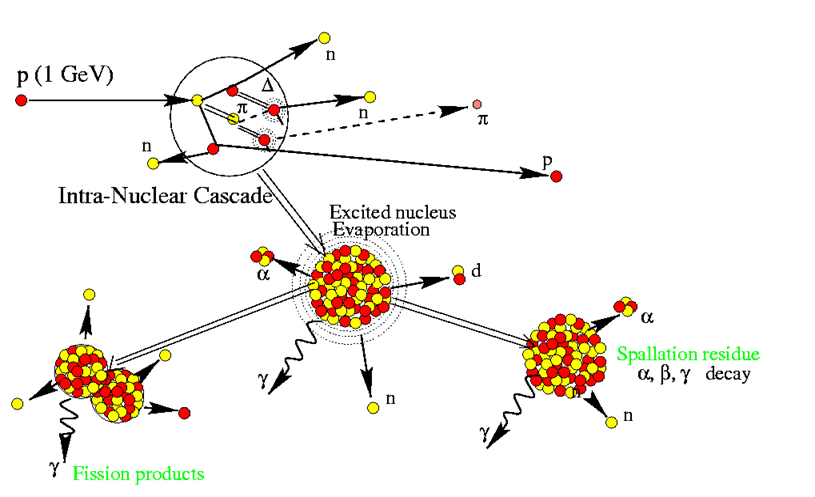
\includegraphics[width=1.0\textwidth]{inclScematic}
}

\subsection{}
\frame{
\frametitle{INCL4.3}
INCL\footnote{A. Boudard, C. Volant, S. Leray, J.C. David (CEA/SPhN),
J. Cugnon, T. Aoust, P. Henrotte (Univ. Li\'{e}ge - Belgium)} provides spallation model
coupled with evaporation and fission models.
\vspace{0.4cm}

\begin{itemize}
\item Possibility to use Geant4 Fermi break-up or
ABLA\footnote{K-H Schmidt, A. Kelic, J. Benlliure GSI and Univ Santiago de C.} 
de-excitation (evaporation and fission).

%\item \todo{Evaporation of light clusters is coming in ABLA07. This is
%  not part of Geant4 yet and we definitely don't have time to
%  translate it in 2009 (the FORTRAN version of abla07 will probably be
%  released in 2009).}

\item Based on physics (phenomenology reduced)
to be predictive.

\item $\sigma(E)$ and $d\sigma/d\Sigma(\theta)$ from experiments,
no ad hoc parameters in the model.

\item Series of elementary scattering explicitly followed in time.

\item Trajectories are straight lines.
\end{itemize}
%REMINDER: There is no $\pi N \rightarrow \pi N$, but it is partly taken
%          into account through $\Delta$ formation and decay.
\begin{center}
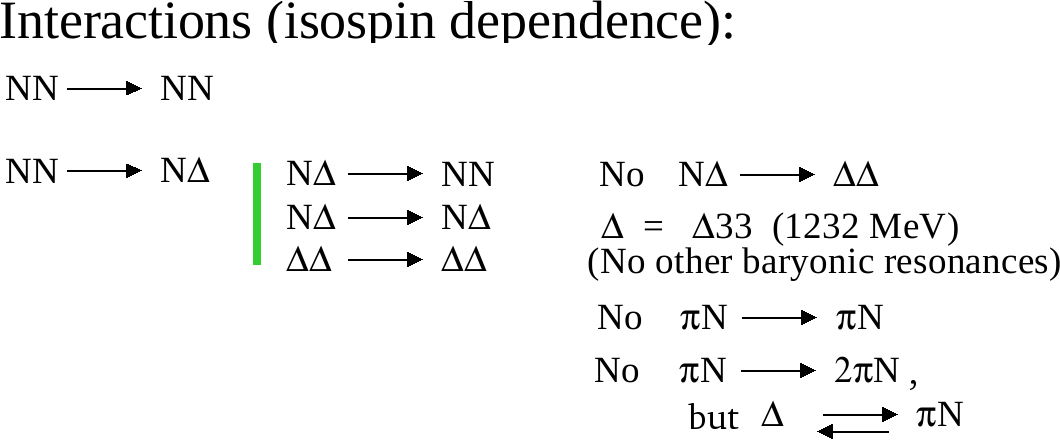
\includegraphics[width=0.6\textwidth]{interactions}
\end{center}
% No piN->piN  but piN<->Delta  
% NOTE: Say that there is no explicit piN scattering but through a 
%       \Delta formation and decay it is partly taken into account.
}

\subsection{}
\frame{
\frametitle{INCL4.3 (cont.)}
\begin{itemize}
\item Pauli blocking on nucleons after each events + long range correlation (CDPP).

\item No collision between spectators, only reflections (cannot escape).

\item Stopping time of the cascade:   $t_{max}= 70.0~\mathrm{fm/c}~(A/208)^{0.16}$.

\item Current version INCL4.3. supports
light cluster production (d, t, $^3$He, $^4$He)\footnote{First version 
       of light cluster production Nucl. Phys. A740 (2004) 195}.

\item All outgoing particles (remnant nucleus, nucleons, pions)
characterised by (A, Z, E$^{*}$, J, P, $\theta$, $\phi$).

\item INCL5 expected year 2010.
\end{itemize}
\begin{center}
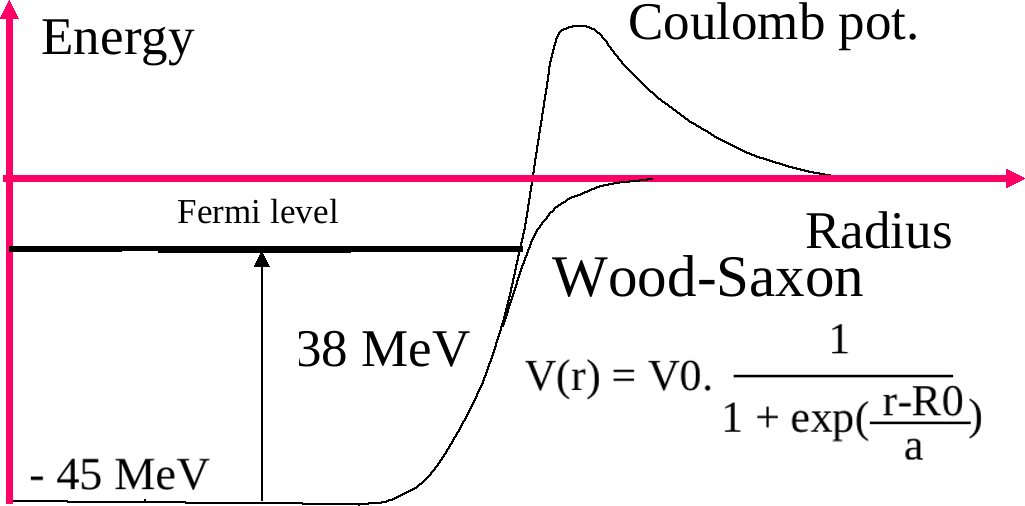
\includegraphics[width=0.6\textwidth]{inclPotential}
\end{center}
}

\subsection{}
\frame{
\frametitle{}
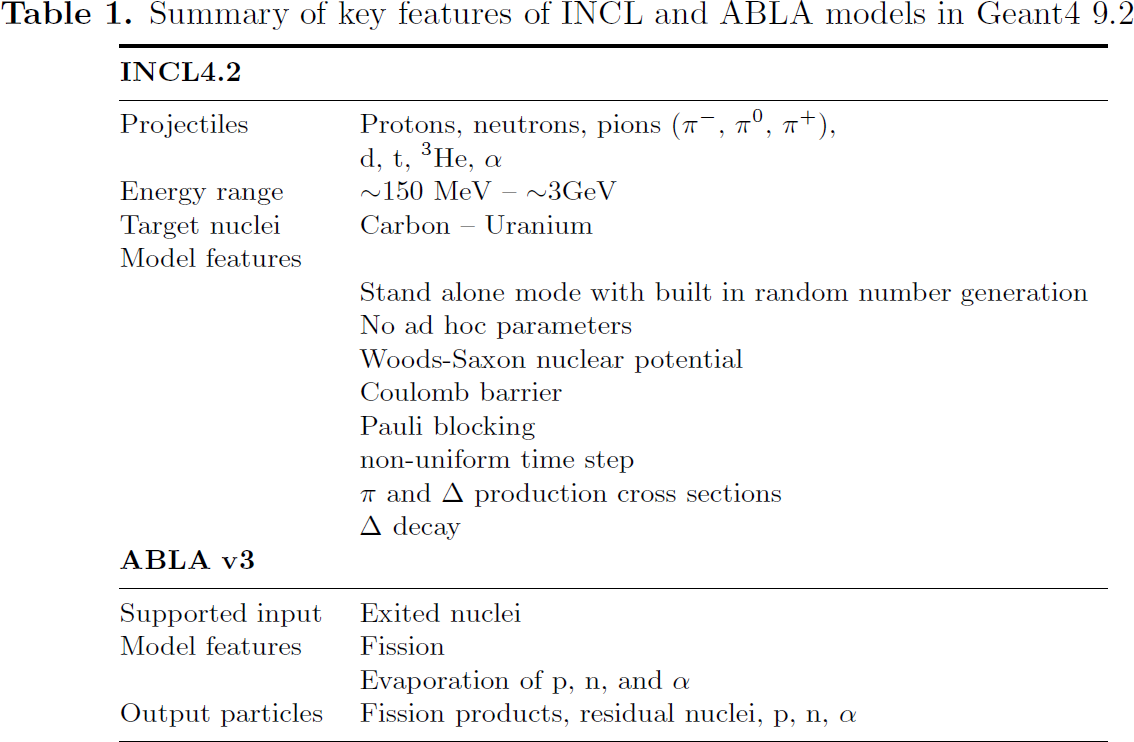
\includegraphics[width=1.0\textwidth]{inclSummary}
}

\subsection{}
\frame{
\frametitle{{\tt QGSP\_INCL\_ABLA} physics list}
A unique feature of Geant4 is to decouple physics models, cross sections, and processes using
abstract interfaces, and manage the usage of different options with so-called the physics lists.

\vspace{0.3cm}
We have prepared a new physics list {\tt QGSP\_INCL\_ABLA} suitable 
for $^{12}$C ion beam fragmentation studies.

\vspace{0.3cm}
\begin{center}
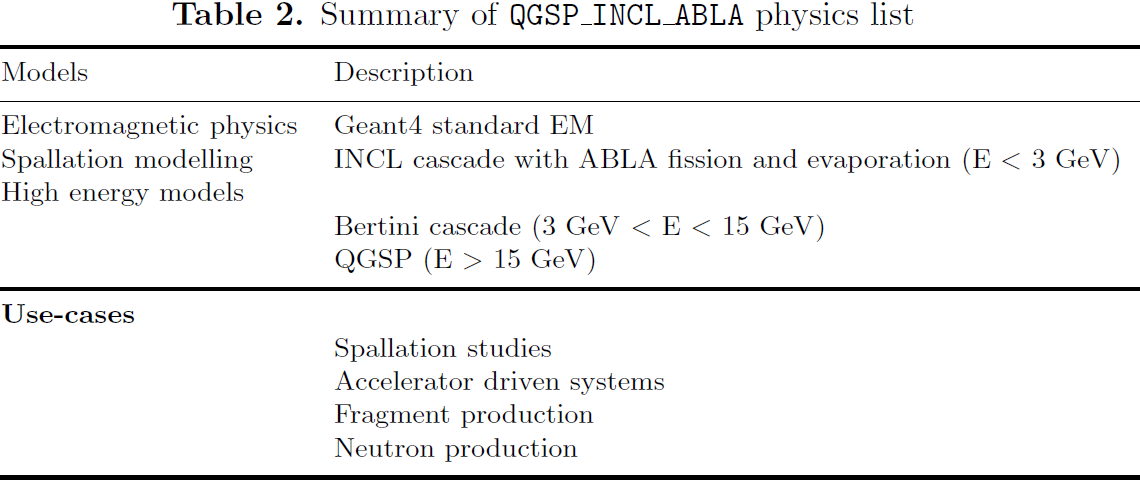
\includegraphics[width=0.9\textwidth]{inclList}
\end{center}
}

\subsection{}
\frame{
\frametitle{{\tt QGSP\_INCL\_ABLA} physics list (cont.)}
First version of the physics list is now available for
IAEA benchmarking~\footnote{Submitted to JPCS May, 2009.}.
\vspace{0.1cm}
\begin{center}

\includegraphics[width=1.0\textwidth]{inclAbstract}
\end{center}
}

\subsection{}
\frame{
\frametitle{Neutron production from proton beam}
\begin{center}
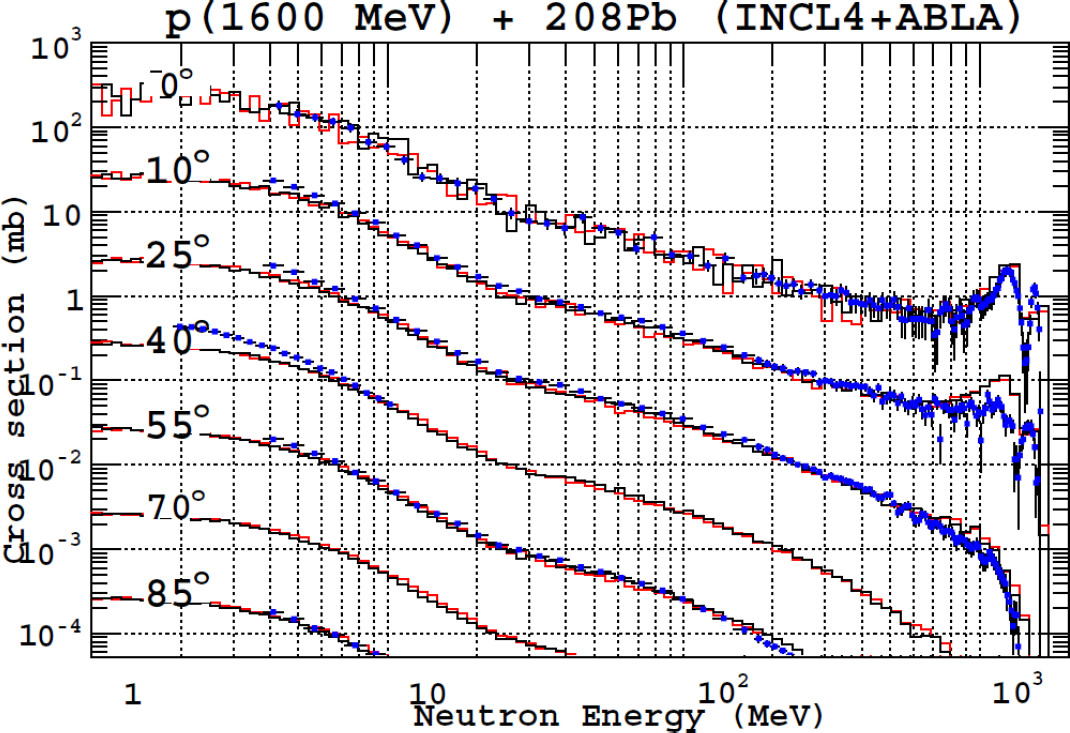
\includegraphics[width=0.8\textwidth]{ddxsec}
\end{center}
}

\subsection{}
\frame{
\frametitle{Example of fragment production}
\begin{center}
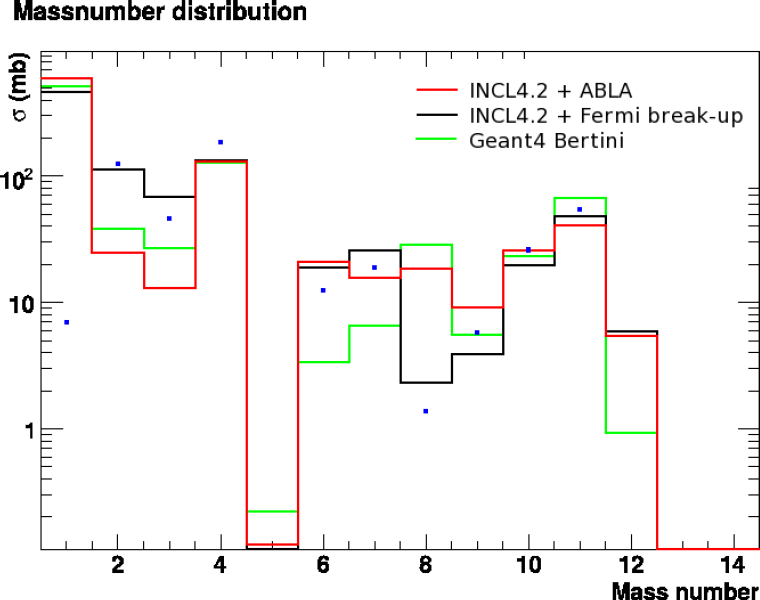
\includegraphics[width=0.6\textwidth]{inverseCbeam}
\end{center}
Comparison of
mass number distributions from
p(1.0 GeV) + C reaction, given by
INCL4.2 cascade with ABLA v3
evaporation and with standard
Geant4 Fermi break up model
against data from~\cite{olson83a}. 
Also, results from Geant4 Bertini cascade with
internal fragmentation model are shown.
}

\subsection{}
\frame{
\frametitle{INCL: Excitation functions}
\begin{center}
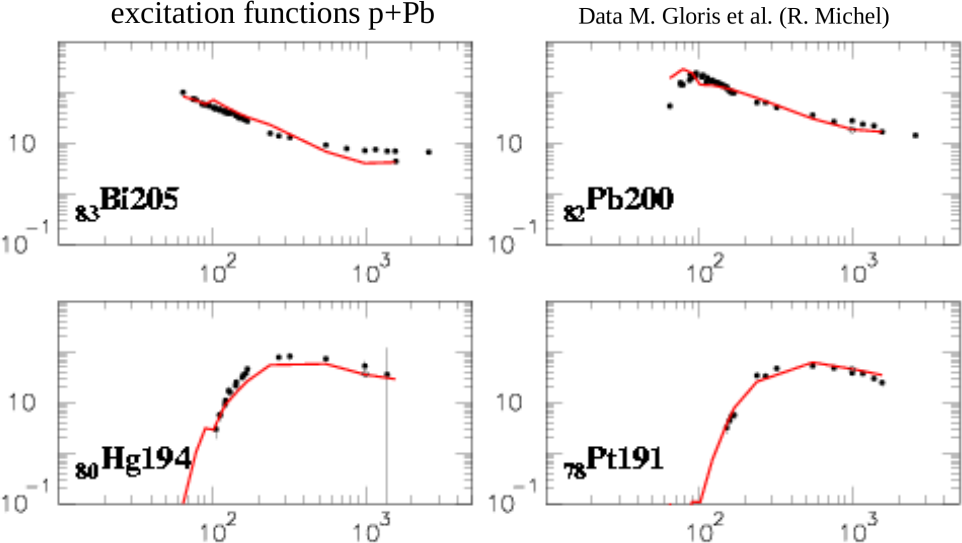
\includegraphics[width=1.0\textwidth]{inclExcitation}
\end{center}
}


%SATO H. et al., Phys. Rev. C 64 (2001) 34607.
\subsection{}
\frame{
\frametitle{INCL + ABLA: Recoil velocity}
\begin{center}
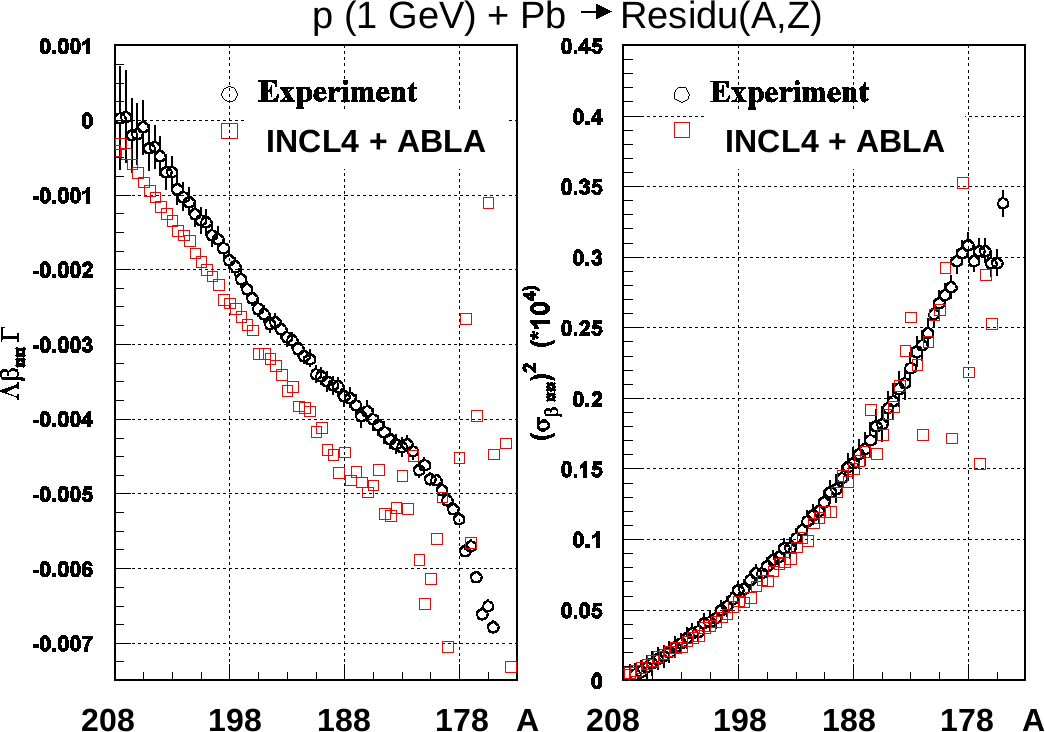
\includegraphics[width=0.8\textwidth]{inclRecoilVelocity}
\end{center}
}

\subsection{}
\frame{
\frametitle{INCL + ABLA : Recoil energy}
\begin{center}
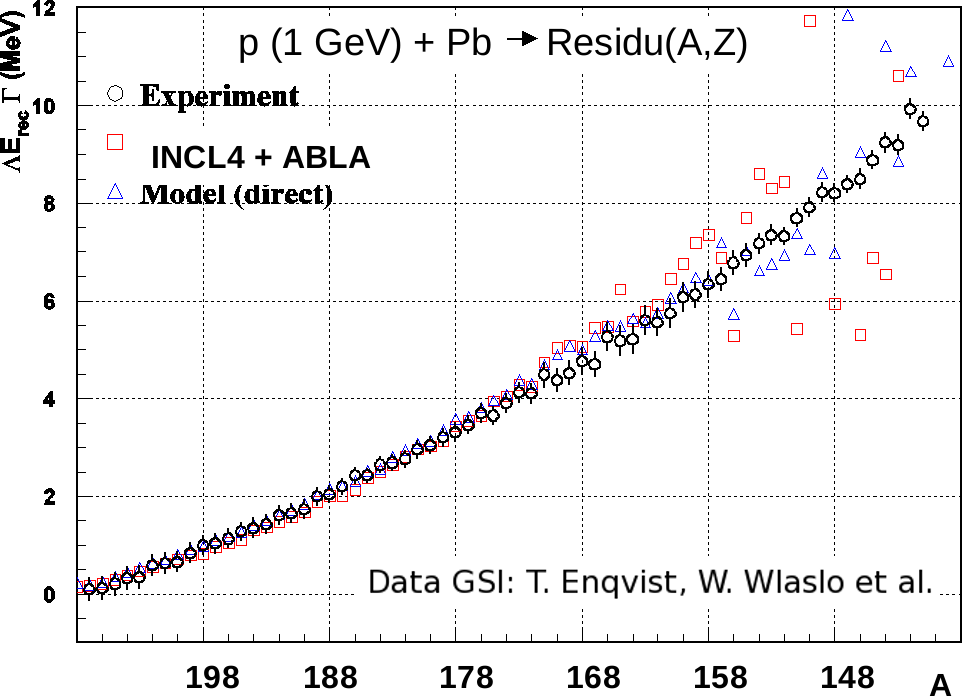
\includegraphics[width=0.8\textwidth]{inclRecoilEnergy}
\end{center}
}

\subsection{}
\frame{
\frametitle{INCL: Light ions\footnote{From \cite{boudard09a}~\attachfile{Acc_App_vienne2.pdf}}}

\begin{center}
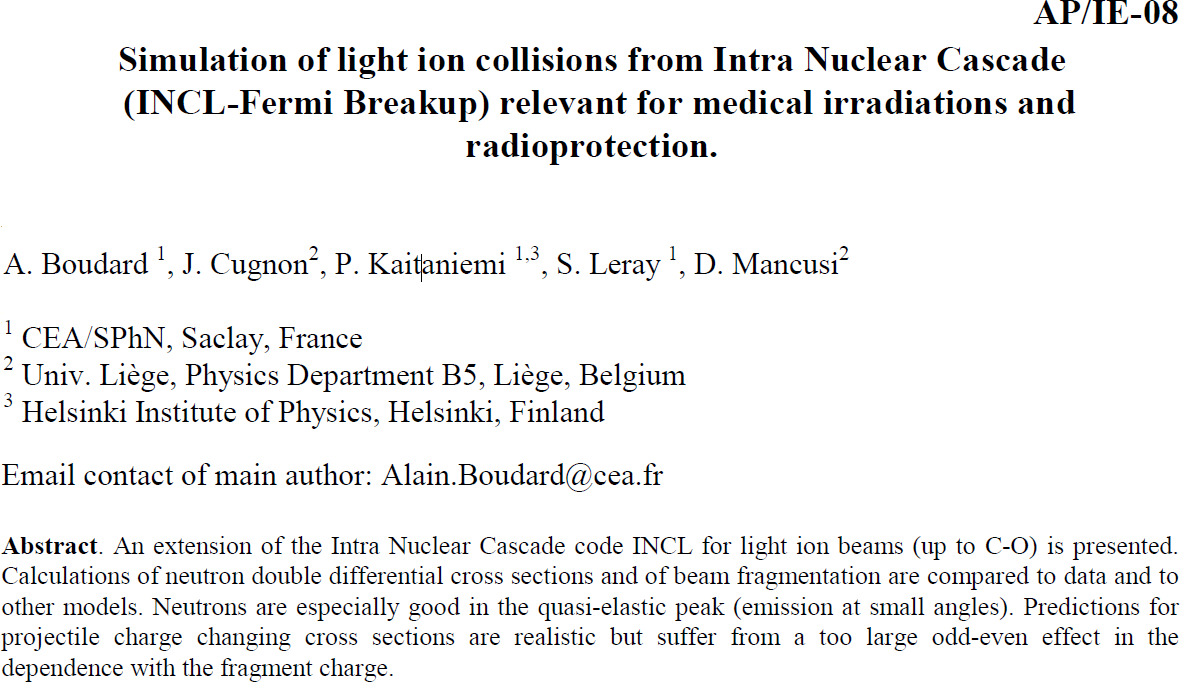
\includegraphics[width=0.9\textwidth]{inclAbstractC}
\end{center}
}

\subsection{}
\frame{
\frametitle{INCL: $^4$He 135~MeV/A + C \footnote{Image from~\cite{boudard09a}. 
                      Data points are from \cite{sato01a}. }}

\begin{center}
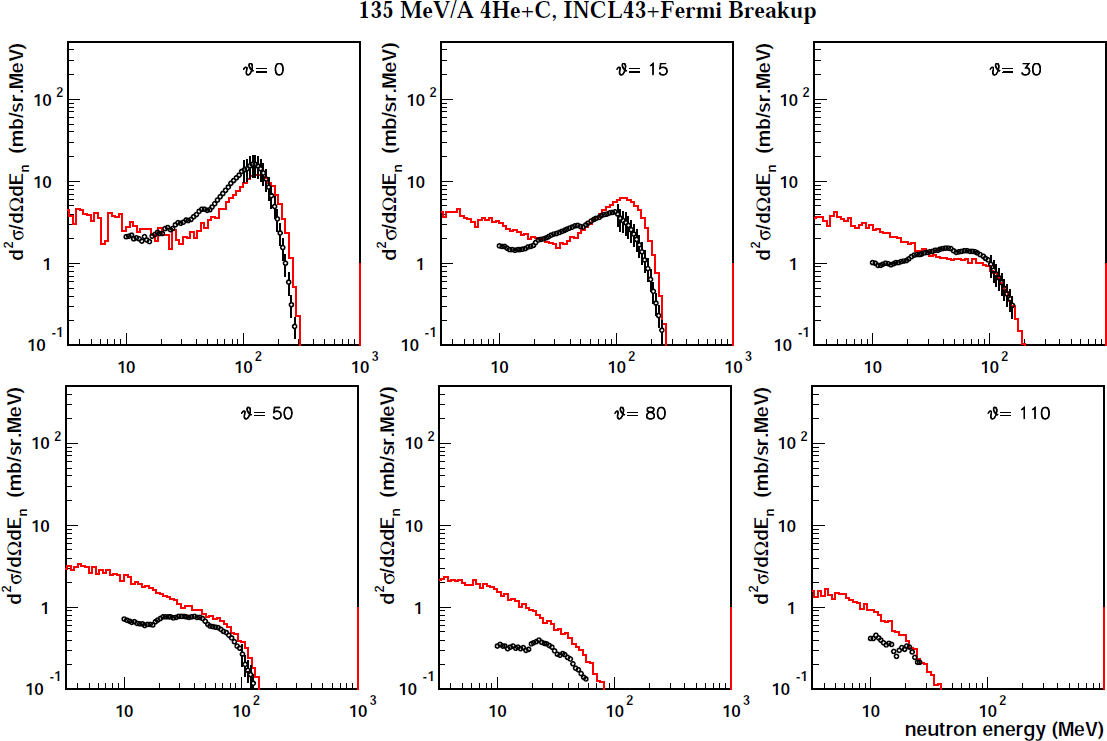
\includegraphics[width=0.75\textwidth]{he135_c}
\end{center}
}

\subsection{}
\frame{
\frametitle{INCL: $^{12}$C 135~MeV/A + C \footnote{Image from~\cite{boudard09a}. 
                      Data points are from \cite{sato01a}.}}

\begin{center}
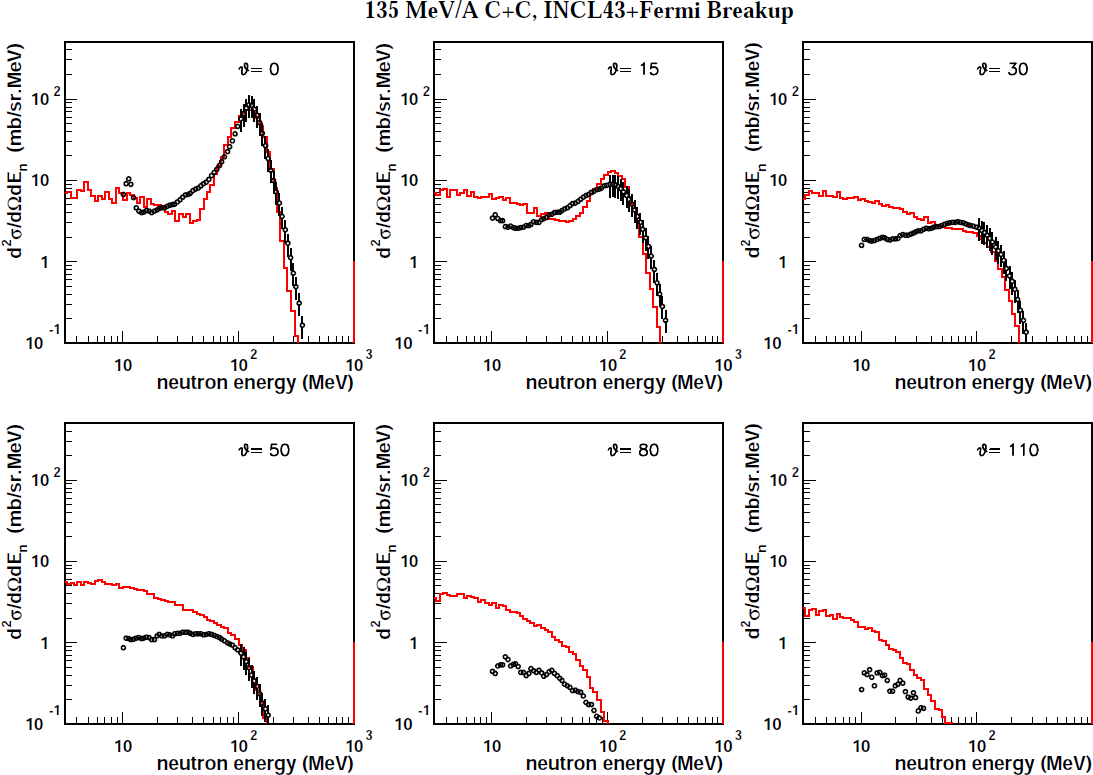
\includegraphics[width=0.75\textwidth]{c135_c}
\end{center}
}

\subsection{}
\frame{
\frametitle{INCL: $^{12}$C 290~MeV/A + C \footnote{Image from~\cite{boudard09a}. 
                      Data points are from \cite{iwata01a}.}}
\begin{center}
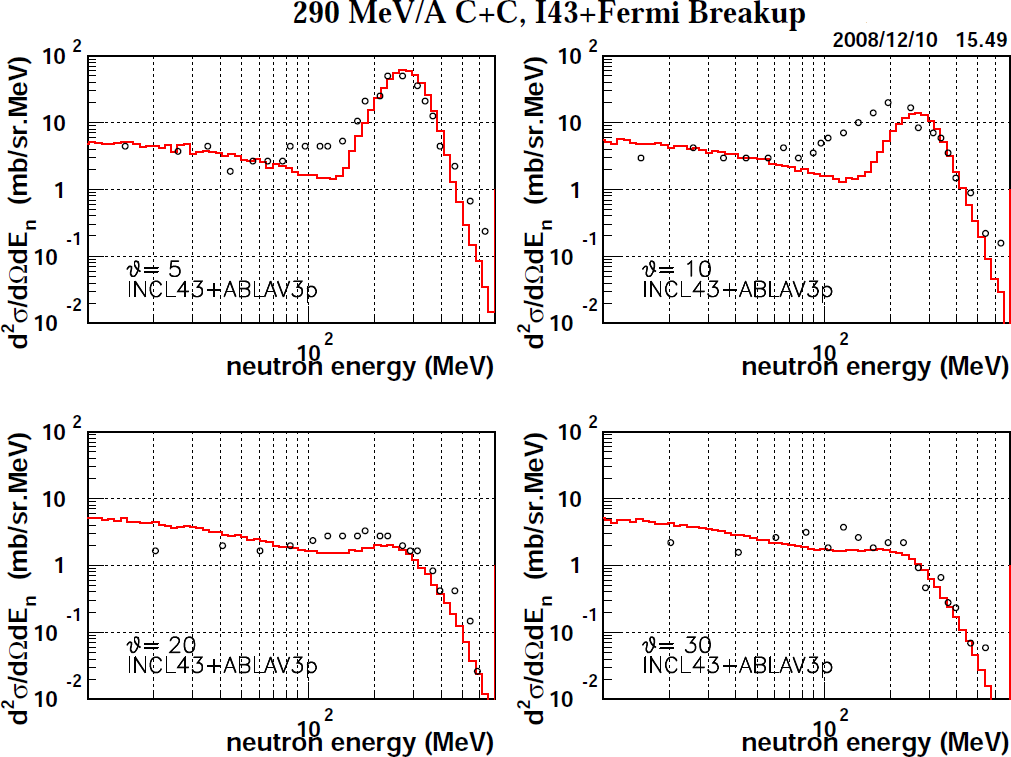
\includegraphics[width=0.75\textwidth]{c290_c}
\end{center}
}

\subsection{}
\frame{
\frametitle{INCL: $^{12}$C 290-400~MeV/A + Cu \footnote{Image from~\cite{boudard09a}. 
                      Data points are from \cite{iwata01a}.}}
\begin{minipage}{5.5cm}
\begin{center}
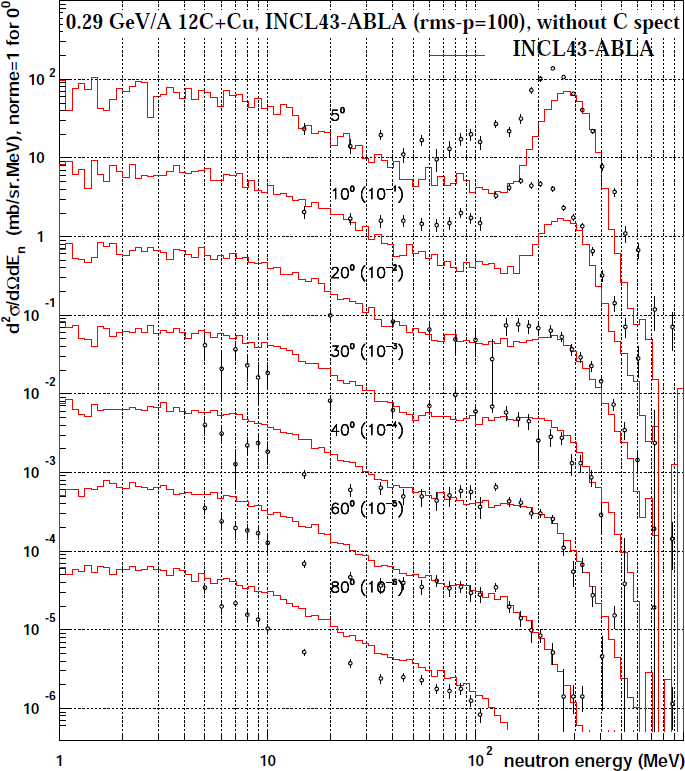
\includegraphics[width=1.0\textwidth]{c290_cu}
\end{center}
\end{minipage}
\begin{minipage}{5.5cm}
\begin{center}
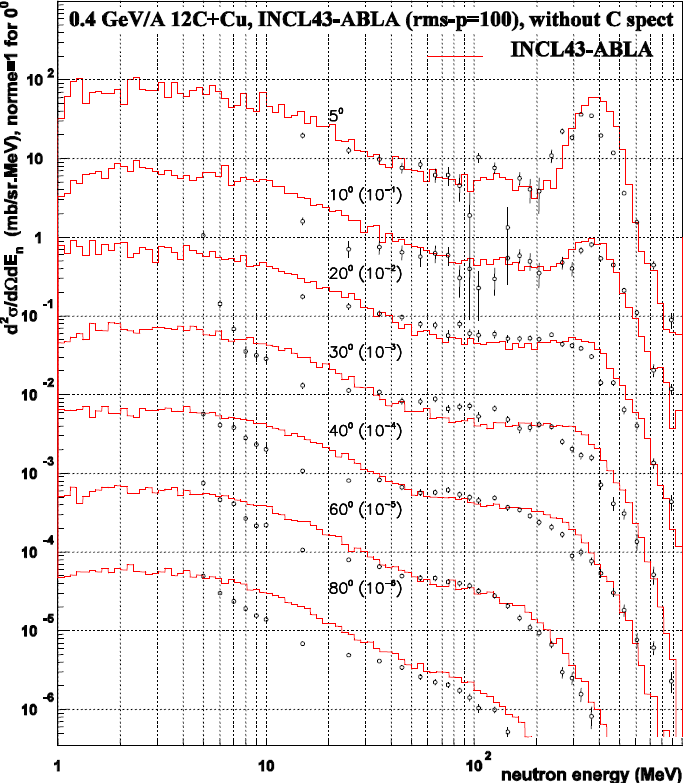
\includegraphics[width=1.0\textwidth]{c400_cu}
\end{center}
\end{minipage}
}

\subsection{}
\frame{
\frametitle{INCL: $^{12}$C 500~MeV/A + Fe \footnote{From \cite{boudard09a}}}
\vspace{0.1cm}
\begin{center}
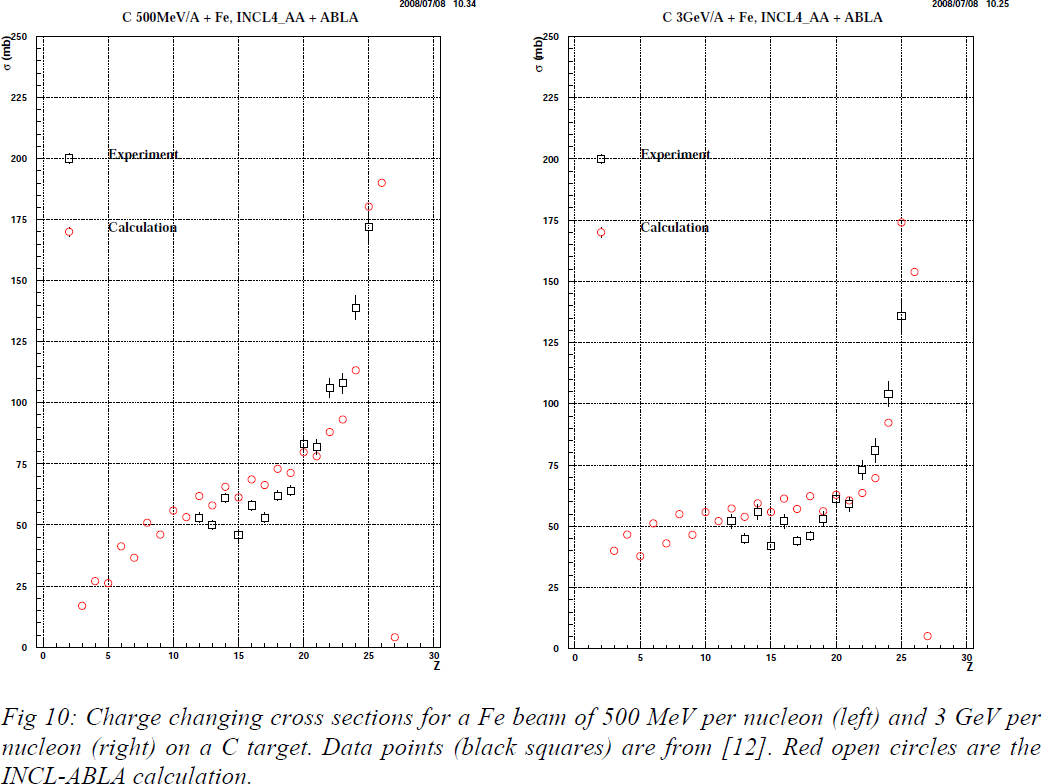
\includegraphics[width=0.75\textwidth]{chargeChanging}
\end{center}
}

\frame{
\frametitle{Examples of physics performance: neutron production from ion projectiles}
\begin{minipage}{5.5cm}
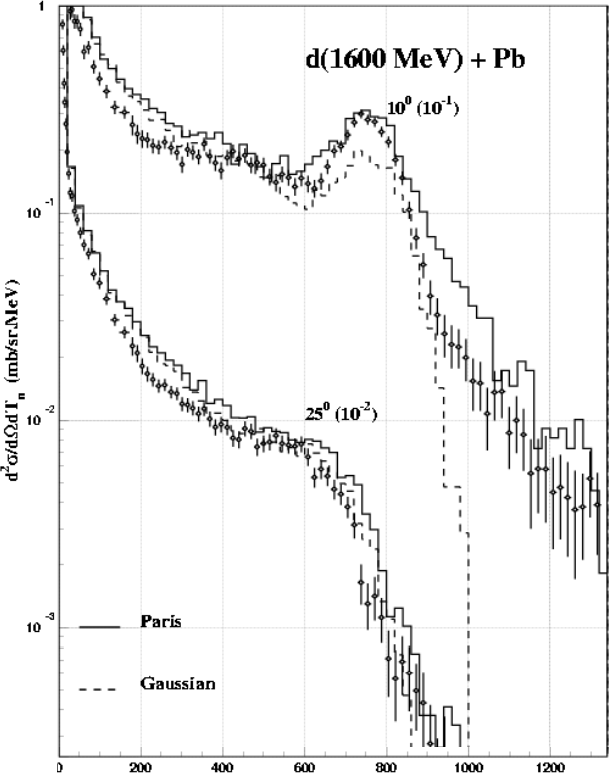
\includegraphics[height=0.77\textheight]{inclDeuterium} % height
\end{minipage}
\begin{minipage}{6cm}
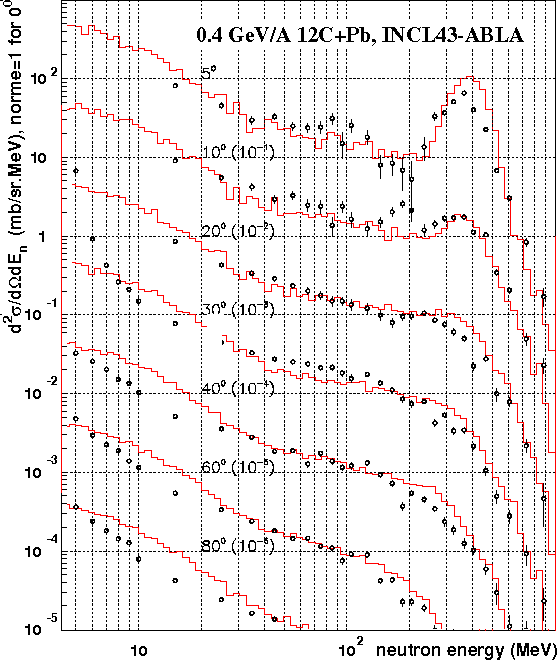
\includegraphics[width=0.96\textwidth]{inclC} % NOTE \textheight 
\end{minipage}
}


\subsection{}
\frame{
\frametitle{Geant4 validation: $^{12}$C beam fragmentation in water target}
%GSI Setup for Angular measurement

We are currently preparing a Geant4 simulation to validate INCL/ABLA models
against data from GSI $^{12}$C beam fragmentation in water target\footnote{Images from 
E. Haettner, {\em Experimental study on carbon ion fragmentation in water using GSI therapy beams},
Master of Science Thesis, Kungliga tekniska h\"{o}gskolan, Stockholm~\cite{haettner06a}.}.


\begin{center}
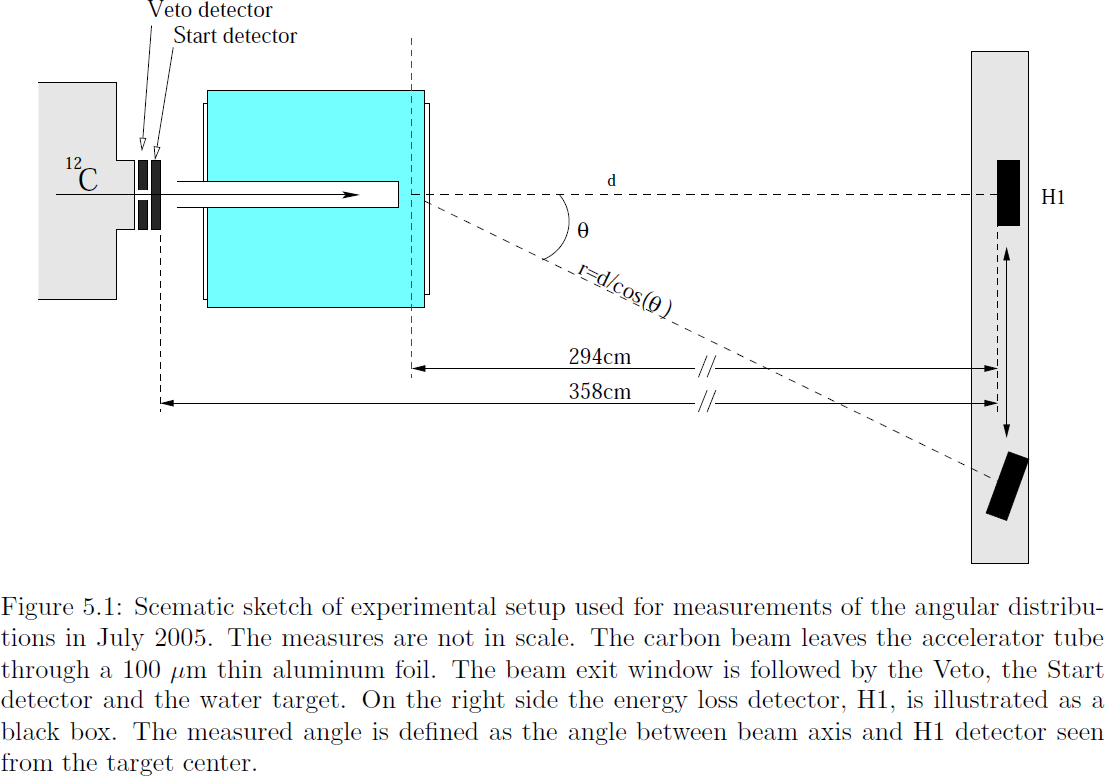
\includegraphics[width=0.60\textwidth]{gsiSetupAngular}
\end{center}
}

\subsection{}
\frame{
\frametitle{GSI experiment: Angular distribution\footnote{Image from~\cite{haettner06a}.}}
First we will compare Geant4 simulation using INCL/ABLA to GSI data and try to reproduce
key plots as published by E.~Haettner 2006~\cite{haettner06a}. 
\begin{center}
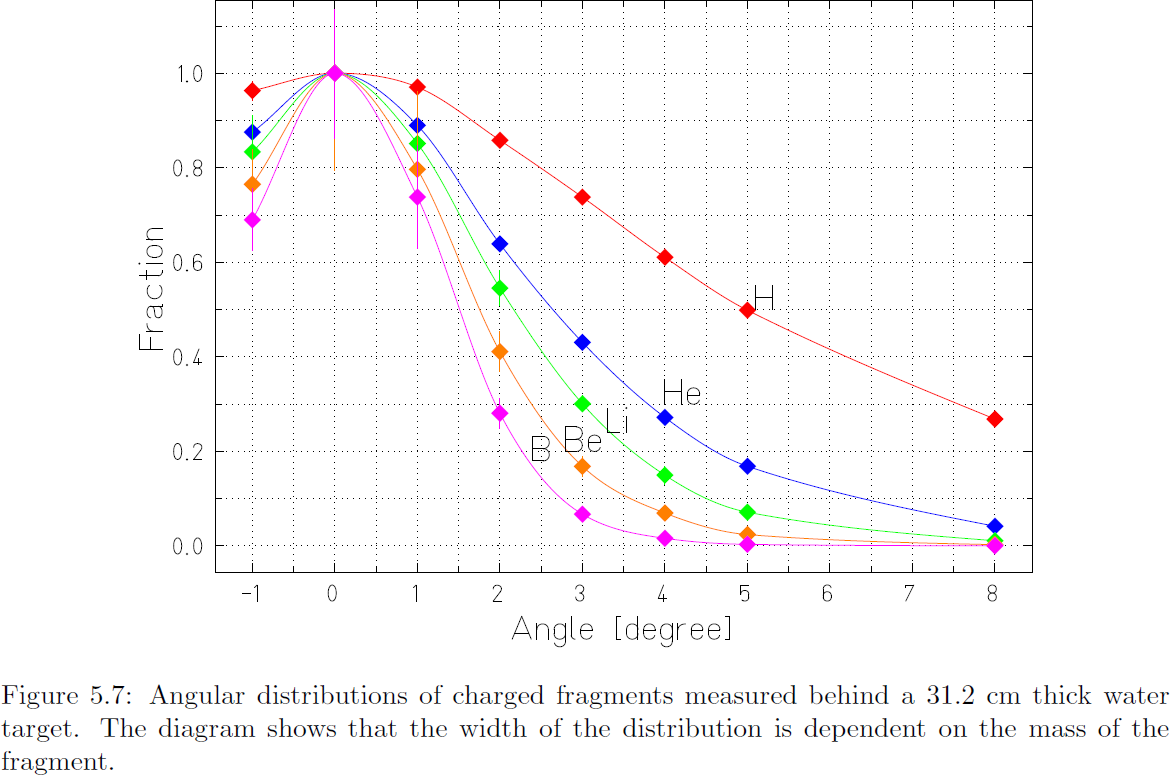
\includegraphics[width=0.7\textwidth]{gsiAngular}
\vspace{0.1cm}
\end{center}
}

\subsection{}
\frame{
\frametitle{GSI experiment: Fragment build-up\footnote{Image from~\cite{haettner06a}.}}
Then, by extending the software tools,  we will prepare IAEA benchmarks for proton and ions as agreed in
the CRP on Heavy Charged-Particle Interaction Data For Radiotherapy.
\begin{center}
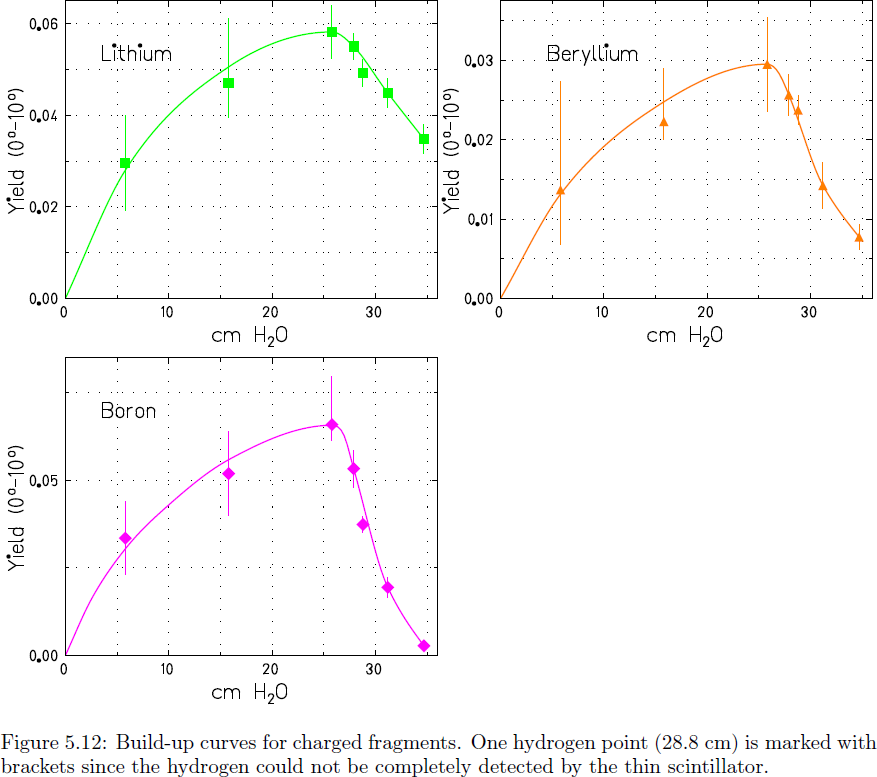
\includegraphics[width=0.54\textwidth]{gsiFragmentBuildup}
\end{center}
}

\subsection{}
\frame{
\frametitle{GSI experiment:  Fragment energy\footnote{Image from~\cite{haettner06a}.}}
 FLUKA simulation already exists, 
so perhaps this could be one benchmark in the CRP,
or similar data set from water target experiment e.g.~\cite{gunzertmarx08a})?	
\begin{center}
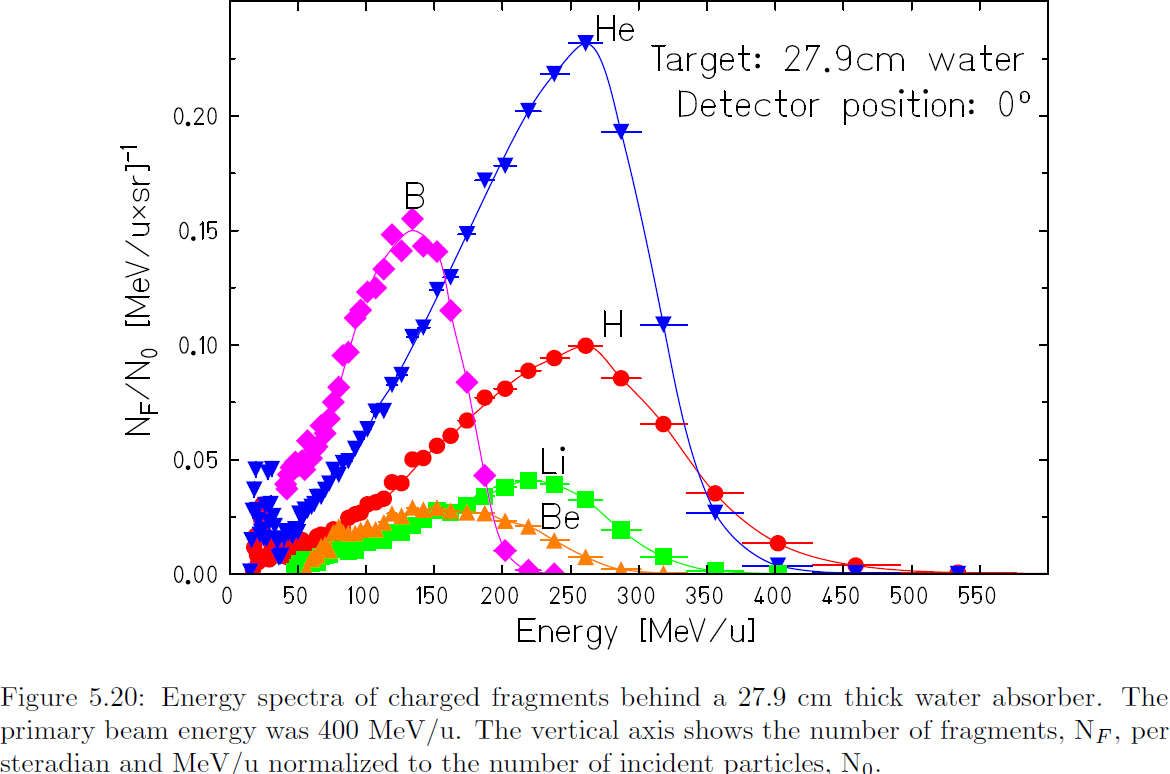
\includegraphics[width=0.65\textwidth]{gsiFragmentEnergy}
\end{center}
}

\subsection{}
\frame{
\frametitle{Implementing the CRP in Geant4}
%\frametitle{GSI experiment: Attenuation and Bragg peak\footnote{Image from~\cite{haettner06a}.}}

\begin{minipage}{6.0cm}
\begin{center}
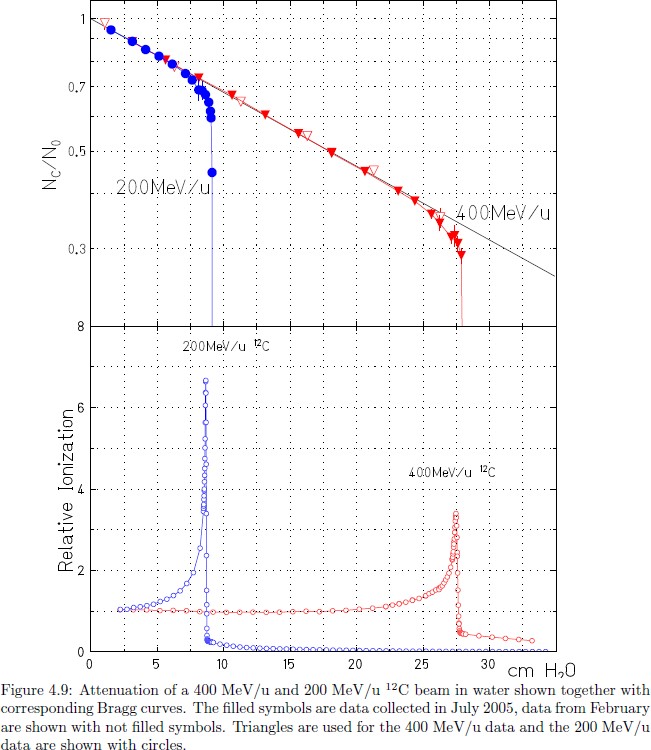
\includegraphics[height=0.70\textheight]{gsiAttenuationBragg}
\end{center}
(Image from~\cite{haettner06a}.)
\end{minipage}
\begin{minipage}{5.5cm}
\begin{itemize}
\item  Our plan is to extend {\bf Hadrontherapy} example (courtesy of INFN-Catania) 
\item Add features, e.g. EXFOR support, from hadron physics {\bf test30} (V. Ivantchenko)
and use extended example as a Geant4 benchmarking platform for 
{\em Heavy Charged-Particle Interaction Data for Radiotherapy.}

\item Simulation is \href{http://github.com/kaitanie/hadrontherapy/}{available in 
open source ditributed Git repository}.
\begin{itemize}
\item Under consideration
\item  Transparent access and possibility to contribute for non Geant4 members 
\item Gateway to Geant4 repository
\end{itemize}
\end{itemize}
\end{minipage}
}

\subsection{}
\frame{
\frametitle{Plans}
\begin{itemize}
\item Geant4 collaboration members from CEA-Sacley, INFN-Catania, J.~M.~Quesada (Universidad de Sevilla), 
and others, will participate to the CRP for compilation and evaluation of 
charged-particle nuclear data for therapeutic applications.

\item We expect to prepare most of our own benchmarks for new Geant4 models INCL4.3/ABLA 
before 2010. (6 months)
\begin{itemize}
\item These Benchmarks will be repeated if INCL5 is available before the end of 2010. (18 months)
\end{itemize}
\item When the platform for agreed IAEA study/benchmarks will have a production quality (3 months)
\begin{itemize}
\item We are prepared to start (3 months) and finish (18 months) agreed proton and ion 
benchmarks for relevant Geant4 models. 
\end{itemize}
%\item Other IAEA Geant4 benchmarks will continue until spring 2010.
\end{itemize}
}

\begin{frame}[allowframebreaks]{References}
\bibliographystyle{alpha}  % Options plain, unsrt, alpha, abbrv
\bibliography{refs} %10 p
\end{frame}
\end{document}

\fi %slides



